\documentclass[11pt, dvipsnames]{beamer}
% If use 16:9 size of beamer, use:
%\documentclass[11pt,aspectratio=169]{beamer}
\usepackage[utf8]{inputenc}
%\usepackage{lmodern}
%\usepackage[T1]{fontenc}
\usepackage{libertine}
\usepackage{libertinust1math}
\usepackage[T1]{fontenc}
\usefonttheme[stillsansserifsmall]{serif}
%----------------------------------------------------------------------------------------
%	SETTING ENVIRONMENT
%----------------------------------------------------------------------------------------

\usefonttheme[onlysmall]{structurebold}%make Navigation Bar font bolder
\usepackage{multicol}
\usepackage{bigstrut}
\usepackage{tabularx}
\usepackage{booktabs}% for much better looking tables
\usepackage{multirow}
\usepackage{amsmath}
%Theme and color  
\usetheme{Boadilla}% more themes, refer to https://mpetroff.net/files/beamer-theme-matrix/
\usecolortheme{seahorse}
\useinnertheme{circles}
\usepackage{enumerate}
\usepackage{graphicx} % Allows including images
\usepackage{caption}
\usepackage{xcolor}
\usepackage{hyperref}
\hypersetup{
	colorlinks=true, 
	linkcolor=black, 
	urlcolor=BrickRed
}

%====Personal information settings====%
\author{Put your name here proudly}
\title[short title]{\textbf{long title of your presentation}}
\subtitle{the subtitle usually follows here}
\institute[NKU]{\textit{Ph.D. Candidate at Department of Political Science, \\ Zhou Enlai School of Government, \\ Nankai University } \\
	\bigskip
	
\includegraphics[width=3cm, height=3cm]{nankailogo.png}}
\logo{
\includegraphics[width=2.5cm, height=0.4cm]{zsglogo.jpg}}
\date{{\tiny \today , Tianjin}}



\setbeamercovered{transparent}
%\renewcommand\thesection{\@Roman\c@section}
\usepackage{romansection}%replace section arabic number with roman number%
\AtBeginSection{\frame{\sectionpage}}
%\setbeamertemplate{navigation symbols}{}%remove nevagation bar blow
%\AtBeginSection[]
%{

%}

%----------------------------------------------------------------------------------------
%	PRESENTATION SLIDES DEPART FROM HERE. ENJOY!
%----------------------------------------------------------------------------------------

\begin{document}
	
	\frame[plain]{\titlepage}
	\begin{frame}
		\textbf{Table of Contents:}
		\tableofcontents
	\end{frame}
	%------------------------------------------------
	\section{\textbf{Short title of section one}\\ \textit{long title of section one, if it's necessary}}
	%-------------------------------------------------	
	\begin{frame}{Outline}
		Put your outline here. 
		\begin{itemize}
			\item The first part of ... is ...
			\item Make clear the question that ...
		\end{itemize}	
	\end{frame}
	%-------------------------------------------------
	\begin{frame}
		\frametitle{Title}
		content...
		\bigskip
		\begin{block}{XXX}
		This is what a block looks like.
		\end{block}
		\begin{exampleblock}{XXX}
		This is what a exampleblock in beamer looks like.
		\end{exampleblock}
		\begin{alertblock}{XXX}
		This is another style of a block.   
		\end{alertblock}
	\end{frame}
	%-----------------------------------------------
	\begin{frame}{\romannumeral1. the title of your part}
		\begin{itemize}
			\item Questionnaire surveys ...
			\item It has been emphasized that ...
			\item ...  
		\end{itemize}	
	\end{frame}
	%-----------------------------------------------
	\begin{frame}
		\frametitle{How to insert tables into your slides?}
		One example follows blow ...
		\begin{table}[htbp]
			\centering
			\scriptsize 
			\renewcommand{\arraystretch}{1.8}
			\begin{tabular}{p{14.72em}|p{25em}}
				\hline
				item & item  \\
				\hline
				item & item \\
				\hline
				item & item \\
				\hline
				item & item \\
				\hline
				item & item \\
				\hline
			\end{tabular}%
			\label{tab:addlabel}%
		\end{table}%	
		
	\end{frame}
	%------------------------------------------------
	\section{The title of your section two}
	%------------------------------------------------- 
	\begin{frame}
		\frametitle{How to insert a picture into slides?}
		\begin{figure}
			\centering
			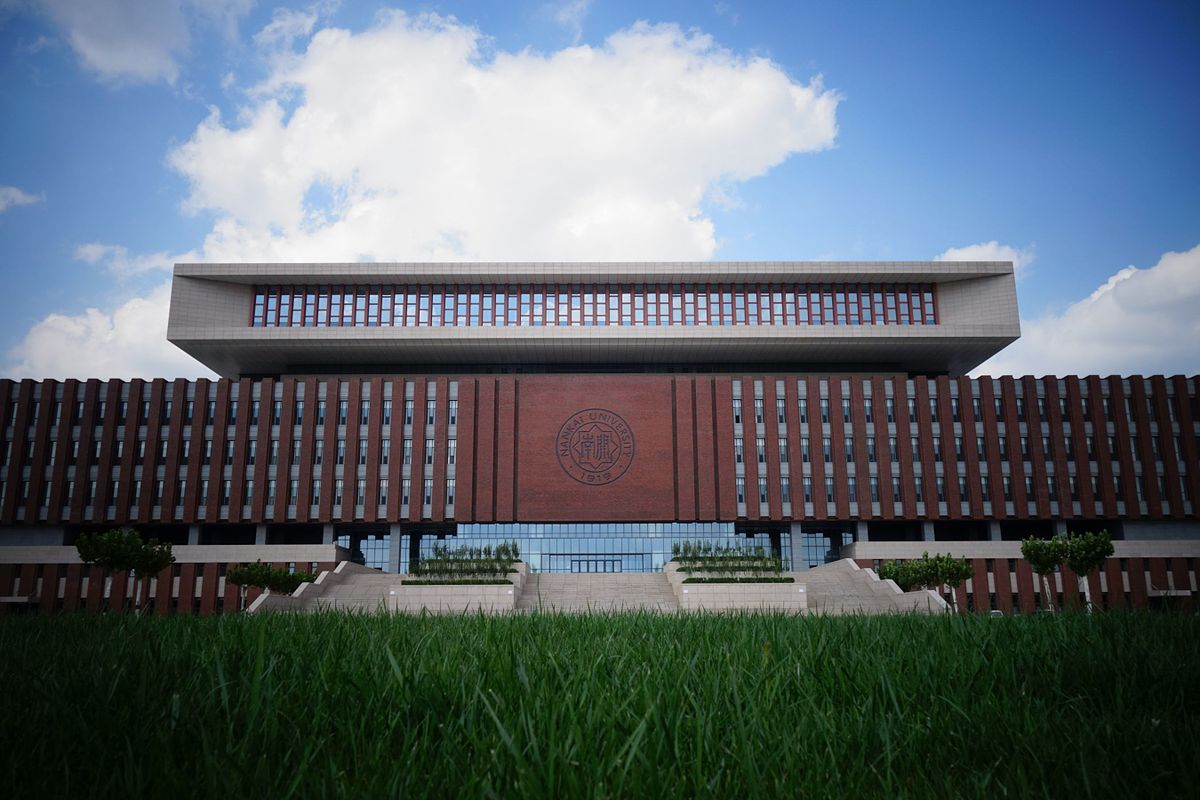
\includegraphics[width=0.7\linewidth]{nkulib}
			\caption{NKU LIBRARY}
			\label{fig:nkulib}
		\end{figure}
		
		\end{frame}
	%------------------------------------------------
	\begin{frame}
		\frametitle{How to insert equation into slides?}
		\begin{equation}
			x = a_0 + \cfrac{1}{a_1 
				+ \cfrac{1}{a_2 
					+ \cfrac{1}{a_3 + \cfrac{1}{a_4} } } }
		\end{equation}
	\end{frame}
	%------------------------------------------------
	\begin{frame}{Acknowledgments}
		\begin{center}
			{
				\Large 
				Thanks for listening! \\ 
				\bigskip
				Q \& A part continues...
			}
		\end{center}
	\end{frame}
	
\end{document}	